\section{Desafio}

\question{Demonstre que o ganho de transresistência $ \frac{v_0}{I_s} $ é o
apresentado a seguir na Figura~\ref{fig:figcircuit}.}
\begin{figure}[H]
  \centering
  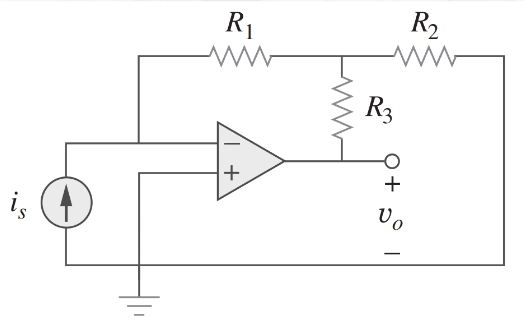
\includegraphics[width=0.4\textwidth]{./fig/circuit.png}
  \caption{Desafio}\label{fig:figcircuit}
\end{figure}
\begin{figure}[H]
  \centering
  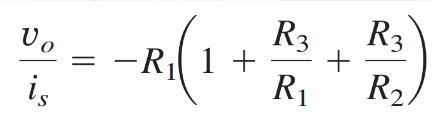
\includegraphics[width=0.4\textwidth]{./fig/vols.png}
\end{figure}
\answer{
  \begin{align*}
    \frac{V_1}{R_1} + \frac{V_1-v_0}{R_3} + \frac{V_1}{R_2}  &= 0 \\
    V_1  &= -i_s R_1 \\
    -i_s R_1 (\frac{1}{R_1} + \frac{1}{R_2} + \frac{1}{R_3}) - \frac{v_0}{R_3} &= 0 \\
    -i_s R_1 (\frac{1}{R_1} + \frac{1}{R_2} + \frac{1}{R_3}) &= \frac{v_0}{R_3} \\
    -R_1 (\frac{R_3}{R_1} + 1 + \frac{R_3}{R_2}) &= \frac{V_0}{R_3} \\
  \end{align*}
}
